%------------------------------------------------------------------------------
%	BIOGRAFIA
%------------------------------------------------------------------------------
\thispagestyle{empty}
\chapter*{Biografia}


\begin{wrapfigure}{l}{3cm} %this figure will be at the right
    \centering
    \vspace{-0.4cm}
    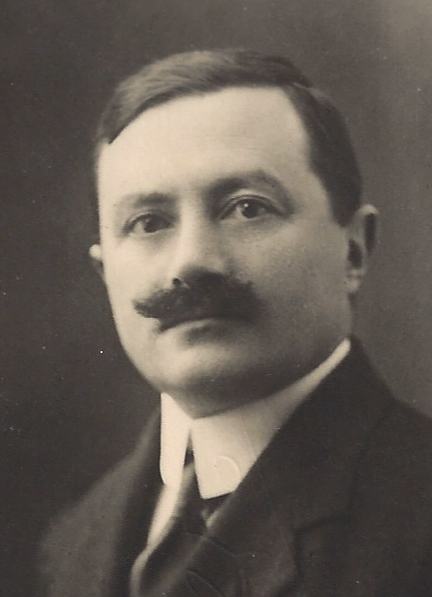
\includegraphics[width=3cm]{mingazzi2}
    \caption[Stefano Mingazzi]{}
    \vspace{-1.1cm}
\end{wrapfigure}
Stefano Mingazzi nacque ad Alfonsine il 3 agosto 1880 da Natale \index[Personaggi]{Mingazzi Natale}Mingazzi (1841 - 1918) e Mariannina Gagliardi\index[Personaggi]{Gagliardi Mariannina (n. 1860)} (1860 - 1882), sorella di Luigi Gagliardi, mio trisavolo. Fu un ricco possidente e fu fascista, non convinto, ma per convenienza. Abitò in Via Reale, all'altezza dell'attuale villa Minguzzi, nella casa appartenuta a suo padre Natale e a suo nonno Fedele. Possedeva un saponificio, vicino al suo palazzo, munito di ciminiera. A fianco al palazzo Mingazzi, vi era l'oratorio padronale San Vincenzo, ancora oggi esistente e chiamato anche Sant'Apollonia per via del quadro raffigurante l'omonima santa all'interno.

Stefano Mingazzi aveva possedimenti nel comacchiese, studiò i territori limitrofi e si appassionò all'ambito della bonifica. Collezionò molte cartine geografiche e molti libri relativi all'argomento, che costituirono la libreria personale di Mingazzi. Scrisse inoltre un libro intitolato "Quattro secoli di pesca nelle valli di Comacchio e l'economia di quel paese" di cui una copia è conservata nella Biblioteca Classense. Ad oggi la collezione di Mingazzi è conservata in parte nella Biblioteca Comunale di Ferrara e in parte nella Biblioteca Classense di Ravenna. La rivista "Il Comune di Ravenna", (fasc. III, 1930, p.34) , dava questa notizia:
\begin{quotation}
  Di speciale rilievo è inoltre il dono bibliografico fatto dal Sig. Stefano Mingazzi. Dalla sua vasta raccolta su Comacchio, messa insieme con sagace diligenza e pazienza di ricercatore, il Sig. Mingazzi ha prelevato circa 73 opuscoli e fogli volanti, di carattere storico letterario, destinandoli alla Classense, che viene così ad accrescere in misura considerevole la sua già ricca collezione bibliografica su quella città che ha tanti rapporti storici con Ravenna. I più degli opuscoli donati sono di un'estrema rarità; qualcuno ormai introvabile.
\end{quotation}
Attorno ai 50 anni si sposò con Amalia \index[Personaggi]{Isani Amalia}Isani, maestra elementare. Siccome non ebbero figli, l'erede biologico di Mingazzi diventò la figlia del cugino di primo grado  Romano \index[Personaggi]{Gagliardi Romano}Gagliardi, di nome Mariannina. Romano fu prigioniero di guerra per quasi tutta la durata dell'infanzia di Mariannina, quindi Stefano diventò quasi come un padre per lei e si prese la responsabilità di crescerla al meglio. Nel 1945 Mariannina ormai diciassettenne, era sfollata insieme alla madre, la nonna e Elio \index[Personaggi]{Marini Elio}Marini che sarebbe stato di lì a poco suo marito. Mingazzi non era d'accordo con questo matrimonio e quindi decise di scrivere un testamento in cui nominava l'Istituto dei Ciechi di Bologna come erede universale di tutte le sue proprietà. La scelta dell'istituto è dovuta al fatto che la nonna di Mingazzi, Andrea Bagnara ved. Gagliardi, morì cieca e sola. Alla fine della guerra, Mingazzi ebbe la possibilità di conoscere Elio Marini e capì che era un ragazzo molto in gamba ed i buoni rapporti furono ben risanati. Tentò più volte di andare a Ravenna per cambiare il testamento, ma essendo stato fascista, il CLN gli impedì di andare a Ravenna per tempi prolungati e lo obbligò a firmare tutti i giorni presso la sede. In questo modo gli fu impedito di cambiare testamento e venne ucciso prima di riuscirci.\\

Il 5 maggio 1945, Mingazzi era già nel suo letto (erano le 23:30), quando delle persone in divisa bussarono. \index[Personaggi]{Lucherini Aldo}Aldo Lucherini, il dottore che aveva il suo ambulatorio nel palazzo Mingazzi, credendo vi fosse bisogno di una visita, aprì. Le persone in divisa chiesero di Mingazzi per portarlo a Ravenna per un controllo, il quale si vestì e andò con loro. Queste persone si erano presentate con un autocarro sul quale vi erano l'industriale \index[Personaggi]{Marini Giuseppe}Giuseppe Marini, \index[Personaggi]{Santoni Corrado}Corrado Santoni e \index[Personaggi]{Santoni Giannino}Giannino Santoni, già prelevati.
\newpage

Nessuno saprà più nulla dei quattro fino al settembre del 1961 quando un contadino, durante i lavori di aratura del suo campo in zona Passetto, vide apparire tra la terra dei resti umani. Erano le ossa appartenute a quattro persone, i cui crani erano bucati dal colpo di un proiettile all'altezza della nuca. Furono trovati anche bossoli di calibro 9 e pezzi di filo di ferro usato per legare le mani ai sequestrati. I famigliari dei quattro prelevati nel maggio del 1945 riconobbero i loro cari da brandelli di vestiti e altri oggetti.

 \begin{figure}[htb]
    \centering
    %\vspace{-0.7cm}
    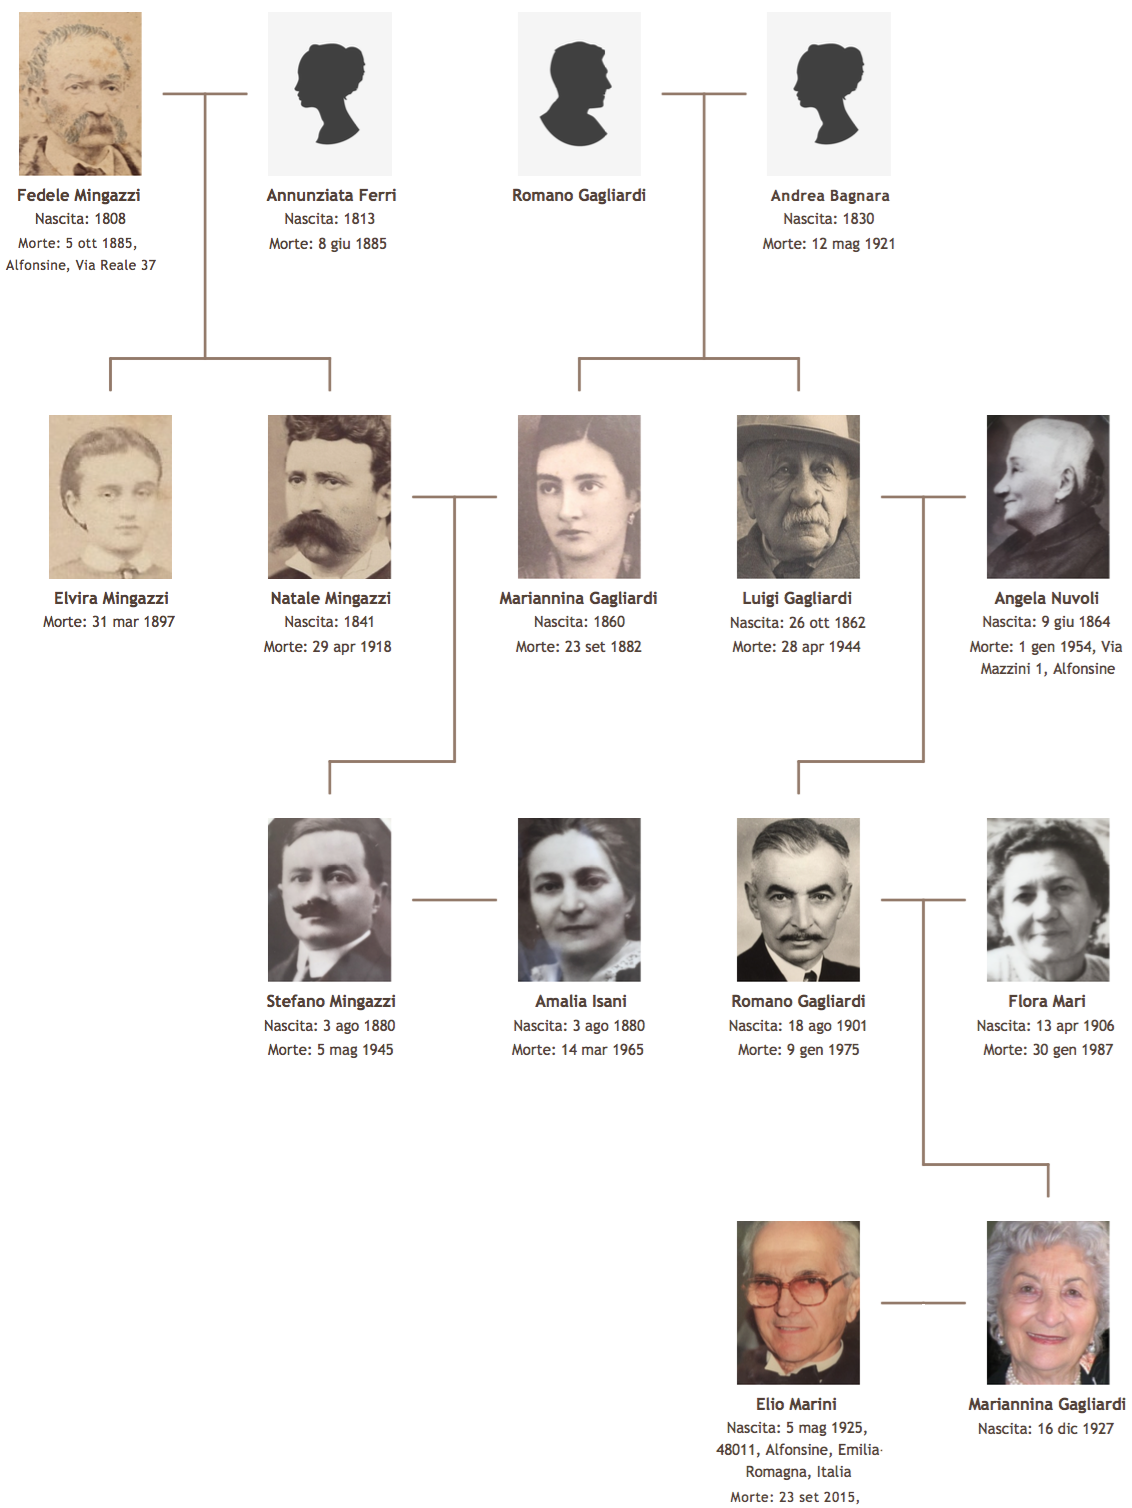
\includegraphics[width=\textwidth]{albero}
    \caption[Albero Genealogico]{L'albero genealogico dei Mingazzi e dei Gagliardi. In basso vi sono i miei nonni, Elio Marini\index[Personaggi]{Marini Elio} e Mariannina Gagliardi\index[Personaggi]{Gagliardi Mariannina (n. 1927)}.}
    %\vspace{-0.3cm}
\end{figure}
